\chapter{Method}
\label{cha:method}

The task of making a better system for labeling clinical reports was approached with different text mining techniques, support vector machines and three learning querying strategies.
At first, the framework and tools used in the system are described, followed by a description of the provided dataset.
Finally, the experiments used to answer the research questions are presented.

\section{Frameworks, Tools and Implementation}
The entire system was written in Python.
The motivation behind this choice was mainly that, when it comes to machine learning and text mining, most of the existing infrastructure at Sectra is using Python.
This, in combination with the fact that there exists several tools for these purposes in Python, such as \textit{numpy} \footnote{Numpy, http://www.numpy.org/}, \textit{nltk} \footnote{Natural Language Toolkit, https://www.nltk.org/}, \textit{scikit-learn} \footnote{scikit-learn, http://scikit-learn.org/stable/} and \textit{gensim} \footnote{Gensim, https://radimrehurek.com/gensim/}.
Most of the plotting was done using the \textit{seaborn} \footnote{Seaborn, https://seaborn.pydata.org/} and \textit{bokeh} \footnote{Bokeh, https://bokeh.pydata.org/en/latest/} libraries.
\textit{pyLDAvis} \footnote{pyLDAvis, https://github.com/bmabey/pyLDAvis} was used for some additional visualization purposes with regards to topic models.

However, when it comes to active learning, there does not seem to be a proven mainstream library that contains a set of readily available algorithms.
In order to achieve better integration between the active learning system and the existing infrastructure at Sectra, as well as making adaptions such as the number of items queried at each iteration, an active learning framework was written from scratch.
The ground for this framework were the algorithms presented in Section~\ref{sec:active-learning}.

This framework consisted of three modules, called \textit{model}, \textit{dataset}, and \textit{query strategy}.
The model is a wrapper around different machine learning models.
By providing an interface for a distance or certainty measure, any underlying model able to provide such an interface can be incorporated.
For accessing the data pool a dataset wrapper was written, with an interface for accessing the labeled and unlabeled pools.
Putting this in its own module opens up the possibility for using several different storage solutions, such as a database or files.
The query strategy module contains the different active learning algorithms for selecting what sample to label next.

\section{Datasets}\label{sec:datasets}

Two different datasets were used in this thesis.
They were the dataset of clinical reports provided by Sectra, as well as Reuters-21578 \footnote{Reuters-21578, https://archive.ics.uci.edu/ml/datasets/reuters-21578+text+categorization+collection}.
The latter was used in order to be able to simulate a multi-label labeling process.
Before being integrated into Sectras system, the different strategies needed to be evaluated from an objective point of view, so that any tradeoffs were known beforehand.
Since the vast majority of the dataset from Sectra was unlabeled, this could not effectively been done using only that.

The set of reports provided by Sectra contained 1068904 different entries, where 493 were initially labeled.
The entries were spread out over several files and stored in the JSON format.
However, those labels were subject to change, so they were mainly used to see if there was a correlation between the labels and clusters during the exploration phase.
A sample report can be seen in Figure~\ref{fig:sample-report}.
The fields include:
\begin{enumerate}
    \item \textbf{ExamId}: The ID of the exam.
    \item \textbf{ReportText}: The text for the report written by the physician after the examination.
    \item \textbf{Anamnesis}: The patient's medical history.
    \item \textbf{PatientAlert}: Anything special about the patient.
    \item \textbf{ExamComment}: Comments regarding the performed examination.
    \item \textbf{Cancelled}: Whether or not the examination was Cancelled.
    \item \textbf{ExamName}: Name of the exam.
    \item \textbf{ExamCode}: Code for the exam.
    \item \textbf{PatientSex}: The sex of the patient.
    \item \textbf{PatientAge}: Age of the patient. This field is truncated if it is above 90 years.
    \item \textbf{Urgent}: If the examination is urgent or not.
    \item \textbf{Pharma}: List of administrated pharmaceuticals.
\end{enumerate}
\begin{figure}
\begin{verbatim}
    {
        'ExamId':       3302250, 
        'ReportText':   '[NUM-SEQ] 
                        Craniell datortomografi utan och med 
                        intravenös kontrast:
                        
                        Frontalt på höger sida finns ett c:a 
                        4 x 3 cm stort lågattenuerande område, tolkas 
                        representera rest efter genomgången 
                        parenchymskada, troligen äldre kontusionsblödning. 
                        Subcorticalt på ömse sidor om centralfåran på höger 
                        sida finns ett några cm-stort lågattenuerande 
                        område som kan vara ischemiskt. Lätt sänkt 
                        attenuering av vit substans periventrikulärt 
                        förenlig med leuko-araios av degenerativ natur. För 
                        åldern normalstora ventriklar. Corticala sulci upp 
                        mot konvexiteten är något smalare än förväntat 
                        för åldern. 
                        
                        Någon tumörsuspekt förändring påvisas ej.',
        'Canceled':     False, 
        'Question':     'Förändring vä temporalt?',
        'PatientAlert': 'Hepatit C-positiv.', 
        'ExamComment':  "Alla kontrastfrågor: UA mnn", 
        'ExamName':     'DT hjärna utan och med iv kontrast',
        'Anamnesis':    'Pat med skalltrauma på 60-talet. Kommer nu med nattliga 
                        från-varoattacker. Skrikigt beteende som tolkats som 
                        epilepsi. CT är aldrig gjort. HEPATIT C-positiv."',
        'ExamCode':     '81081', 
        'PatientSex':   'MALE', 
        'PatientAge':   59, 
        'Urgent':       0, 
        'Pharma':       [{"ExamId": 3200240, "Units": "100 ml", 
                        "Pharma": "Omnipaque Inj.lösn 300 mg I/ml"}]
    }
\end{verbatim}
\caption{A sample report from the dataset provided by Sectra}
\label{fig:sample-report}
\end{figure}

The work was mainly concerned with the ReportText field, since it contains the response to the result of the examination.
But the for the complete Active Learning system the Anamnesis was used as well.
The labels that were initially assigned to these reports were:
``Blödning'', ``Infektion'', ``Metabol'', ``Tumör'', ``Cysta'', ``Missbildning'', ``Syndrom'', ``Demens'', ``Hydrocefalus'', ``Infarkt'', ``Kärlsjukdom'', ``Trauma'', ``Systemsjukdom'', ``Inklämmning'' and ``Normal''.

The distribution of labels among these initially labeled reports can be seen in Figure~\ref{fig:class-distribution}
Note that this is only a count of the individual labels, and the multi-label nature of the labeling is not taken into account in the plot.

\begin{figure}
    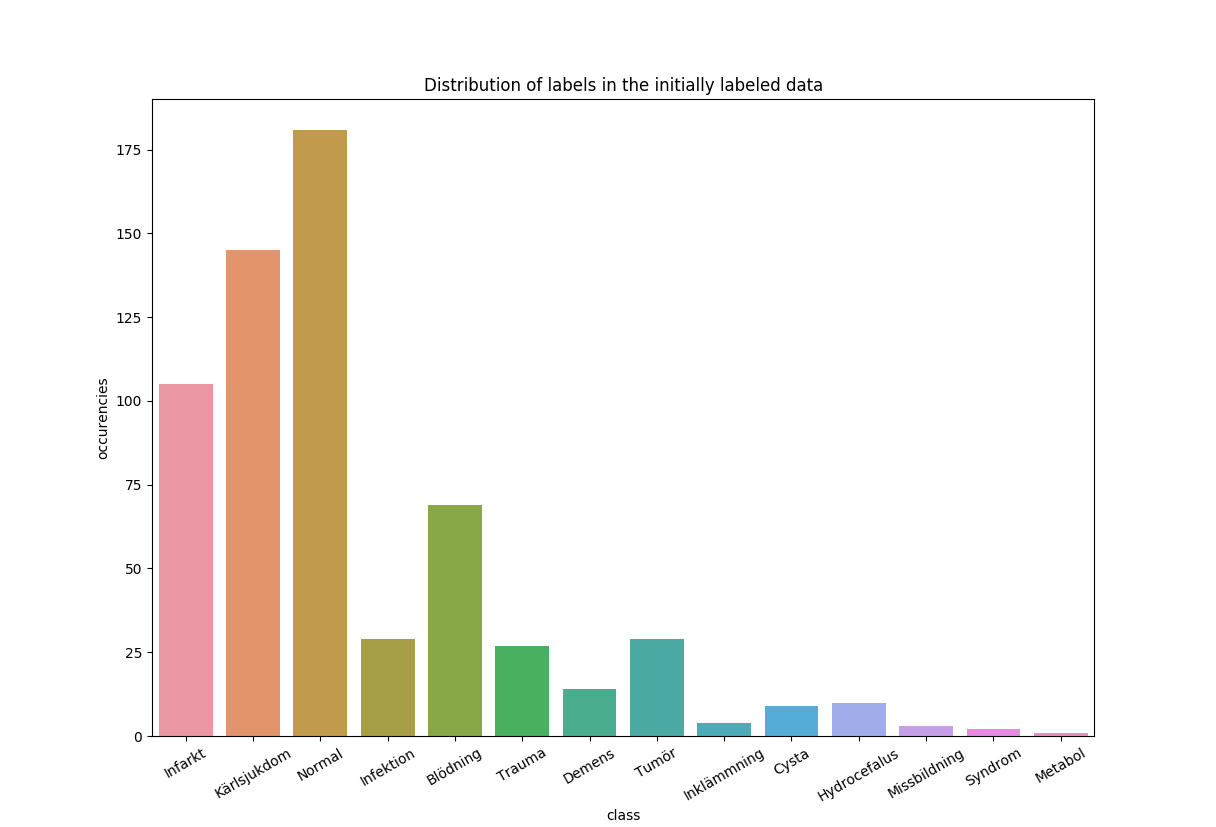
\includegraphics[scale=0.5]{figures/class-distribution.png}
    \caption{The distribution over the labels in the initial set of labeled data provided by Sectra}
    \label{fig:class-distribution}
\end{figure}

The Reuters-21578 newswire dataset is widely used when it comes to text classification research, and provides a good multi-label benchmark that can be used to compare how well certain techniques perform to other papers.
All experiments used the \textit{ModApte} split of the dataset, which is commonly used and readily available. %TODO: Footnote with the dataset?
It splits the dataset into a predefined set of training and test documents, containing 7.769 and 3.019 entries respectively.
This split contains a subset of the categories, specifically 90 different ones.
Since the clinical dataset from Sectra only contained 15 different categories, this would not mirror that very well, so instead the 15 most common categories of those were taken out.
The distribution of the top 15 Reuters-21578 categories can be seen in Figure~\ref{fig:class-distribution-reuters}.
After filtering out the documents not labeled with any of the top 15 categories, there were 6880 documents left in the training set, and 2646 in the test set.

\begin{figure}
    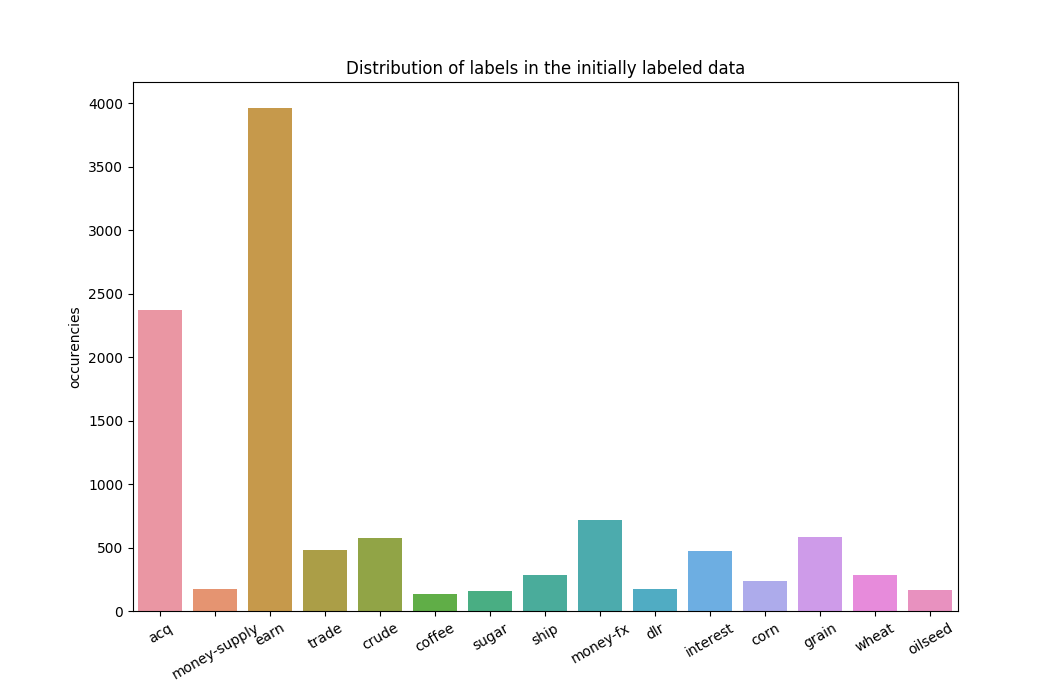
\includegraphics[scale=0.6]{figures/class-distribution-reuters.png}
    \caption{The distribution over the labels in the Reuters data}
    \label{fig:class-distribution-reuters}
\end{figure}

\section{Pre-Processing and Text Representation}\label{sec:pre-processing}

Before the data was used in the conducted experiments, several pre-processing steps were applied in order to clean the dataset and make it easier to work with.
The steps were:
\begin{enumerate}
    \item The first step was to extract the fields of interest.
          For the exploratory phase, and for the use of active learning techniques these were ``ReportText'' and ``Anamnesis''.
          When it came to filter out invalid reports, the ``ReportText'' was the only field of concern.
          It describes the results of the examination, and therefore if there was an examination at all.
    \item White space and punctuation were stripped from the data.
    \item All words were transformed into lowercase.
    \item The most common words as well as very infrequent words were both filtered out.
          Specifically, words occurring in less than 1\% of the documents, and words occurring in more than 90\% were removed.
          The idea behind this is that these words would not contribute to differentiating different classes of documents.
          Removing of both frequent and infrequent words is commonly done when working with text and has been done in the context of classification, active learning or topic modeling before~\cite{tong2001support, blei2003latent, brinker2006active, sarioglu2013topic}.
    \item A list of identified common stopwords were removed as well.
          This list of words was based on the Swedish nltk stopwords list.
          After iterating over the dataset words that occurred frequently but were not considered to be very informative for the models were identified.
          The list of stopwords was then extended to incorporate these words as dataset-specific information.
          For example, this included names of the doctors that had written the report.
          By removing names of doctors the idea is to make the system more applicable to new reports, written by other doctors.
    \item Accents from the words were removed.
    \item The text was tokenized and then stemmed using the swedish Porter2 stemmer \footnote{Swedish Porter Stemmer, http://snowball.tartarus.org/algorithms/swedish/stemmer.html}.
\end{enumerate}
Most of these steps have been performed in previous research  dealing with text analysis in the form of classification or active learning~\cite{tong2001support, blei2003latent, brinker2006active, sarioglu2013topic}.

After transforming the text into a sequence of tokens, the final step before using it with the models was to create a representation that would be beneficial to work with.
The representation chosen was bag of words, i.e. a matrix of tokens count.
Each document is represented by the counts of each token, disregarding the order of the tokens.
In order to get some positional information into the representation additional tokens are stored. 
The additional tokens are bigrams, which are pairs of tokens (i.e. processed words).
By storing the frequency of how often such a pair occurs in the document, alongside the regular one word tokens, some positional information is retained.

\section{Exploratory Study}\label{sec:exploratory-study}
For the exploratory study we used the representation described in Section~\ref{sec:pre-processing}, but without the bigrams.
The main goal of this phase was to get to know and to better understand the dataset.
A part of this goal was to go through the fields for the different reports to see how they worked and what values could be expected.
In order to visualize the data in a 2D plot, t-distributed stochastic neighbor embedding (t-SNE) was used.
It is a dimensionality reduction technique, that is able to transform high dimensional data into two dimensions, trying to retain as much variance as possible.

The first step was to fit an LDA model to the data.
For the purpose of exploring the data, the number of topics were chosen to be a 100, with the hope of it not resulting in too granular topics that would be hard to manually analyze
A 100 topics is what is in the middle of the range Chang et al\@.~\cite{chang2009reading} used for evaluating the interpretability of topics.
Since the purpose of this is only to explore the data, it seemed like a sufficient starting point.
The data points were plotted in a 2D plot after reducing the dimensions using t-SNE.
Each data point was colored based on some trait that the specific data point had.
For the exploratory study, the topic with the highest probability for a given data point was used to determine the color.
A plot of this can be seen in Figure~\ref{fig:lda-dist}.
Although it might be hard to interpret as a 2D plot in this report, the bokeh library allowed for the generation an interactive plot.
Hovering over each data point would show the content of the report and the topics assigned to it, making it a convenient way to explore the data and the generated topics.

\begin{figure}
    \centering
    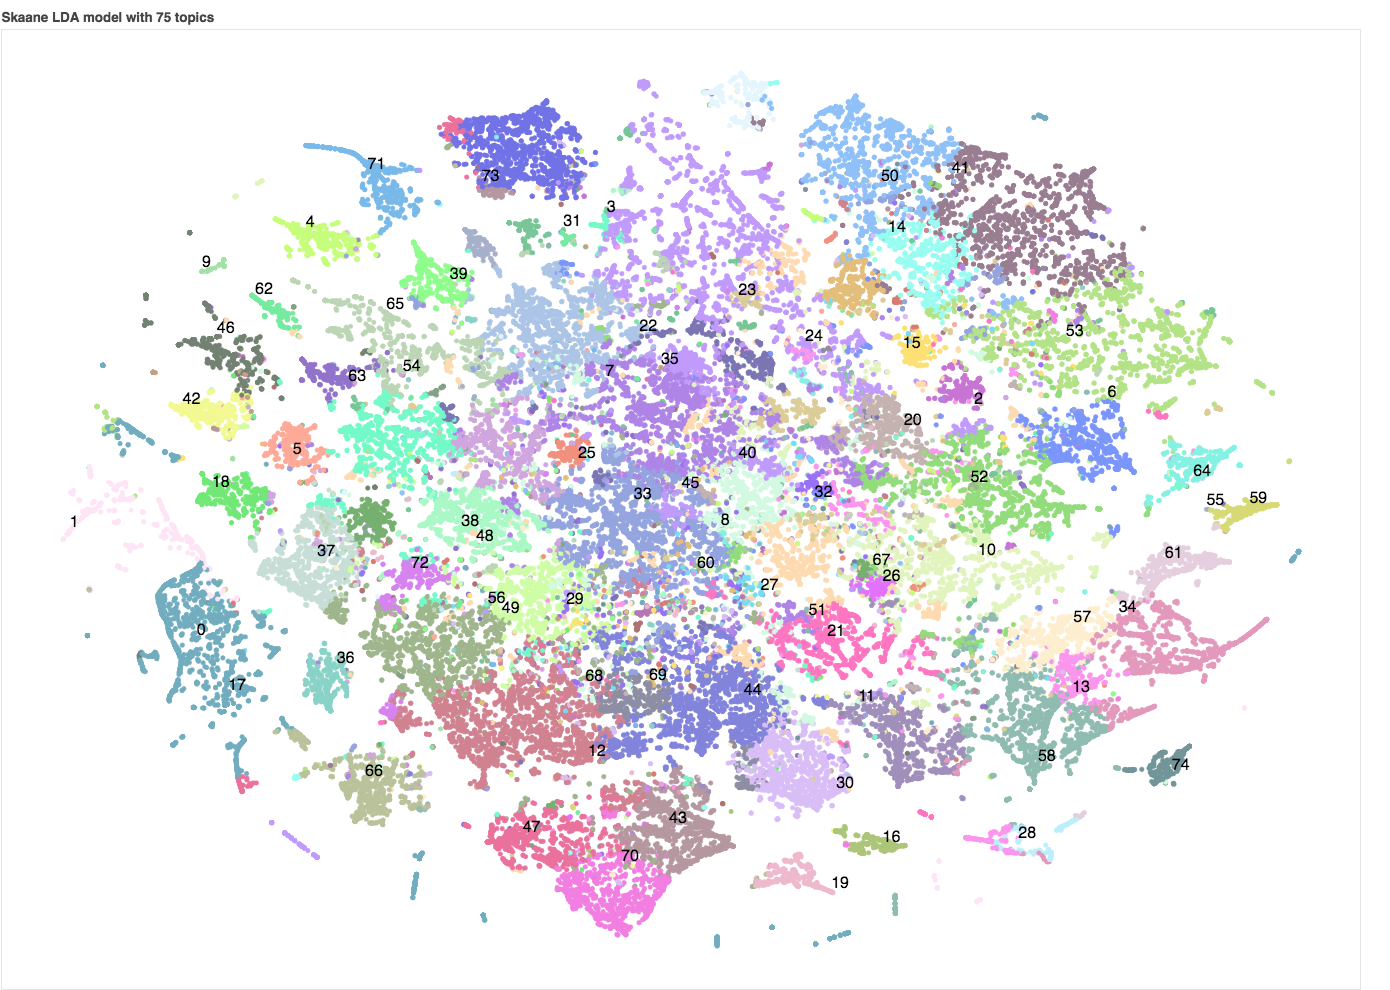
\includegraphics[scale=0.25]{figures/lda-2d-distribution.png}
    \caption{A 2D plot of the text data, where each point is colored by topic with the highest probability}
    \label{fig:lda-dist}
\end{figure}

Samples of the generated topics can be seen in Figure~\ref{fig:topic-wordclouds}.
Another way to visualize the topics for inspection is using the techniques described by Sievert et al\@.~\cite{sievert2014ldavis}.
They propose a \textit{relevance} measure where the probability for a certain term within a topic is weighted against how common that topic is in the entire corpus.
The interactive interface provided by pyLDAvis can be seen in Figure~\ref{fig:ldavis-sample}.

\begin{figure}
    \centering
    \thirdsubfigimg{wordcloud-1}{A wordcloud over the words occurring in topic 1 for an 75 topic LDA model.}
    \thirdsubfigimg{wordcloud-17}{A wordcloud over the words occurring in topic 17 for an 75 topic LDA model}
    \caption{Wordclouds for a 75 topic LDA model}
    \label{fig:topic-wordclouds}
\end{figure}

A word2vec model was used on the entire dataset to evaluate see the relationship between terms and find possible synonyms.
In order to find synonyms, all words in the dataset that had a similarity over 95\% were manually inspected.
In addition to finding synonyms, this model was used to identify names and other identifiers in the reports.
They would come up as similar entities from the model.
Accomplishing this was done by exploring the data through an interactive plot, after using t-SNE to reduce the number of dimensions.

\begin{figure}
    \centering
    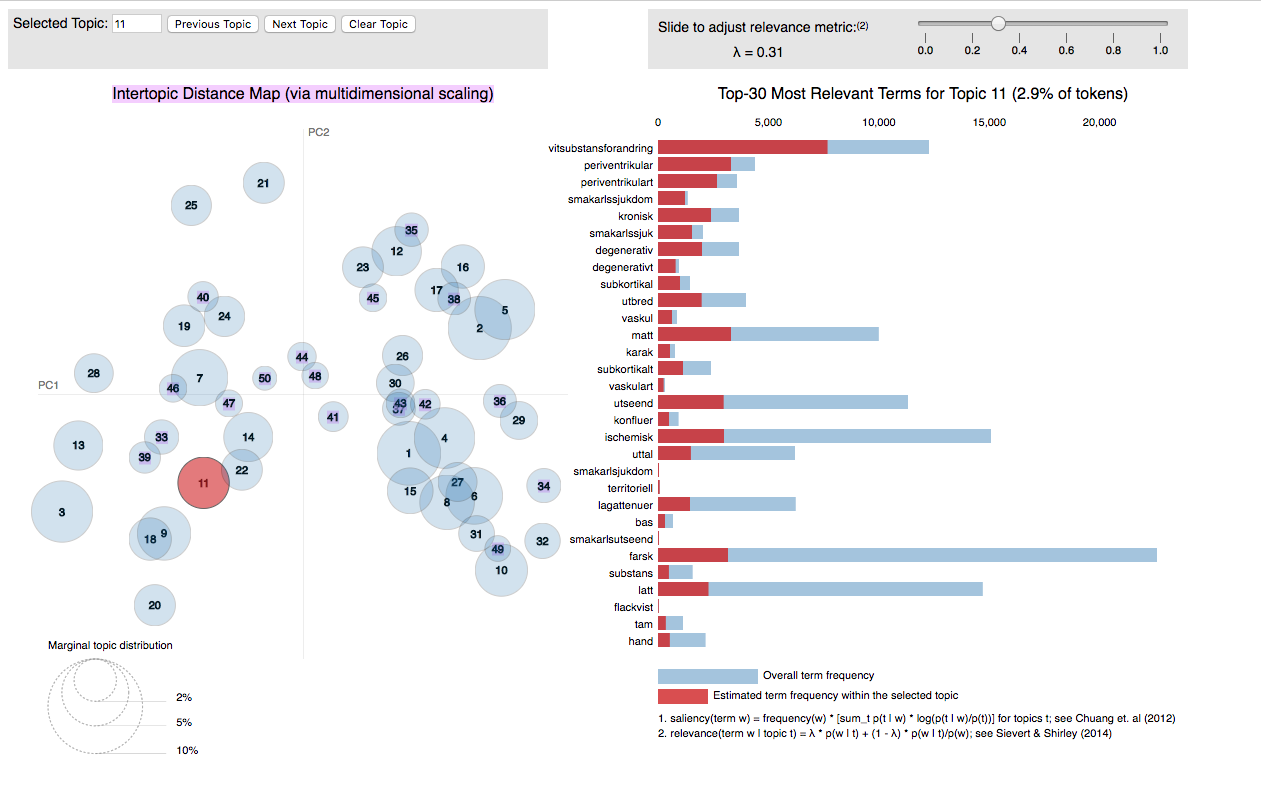
\includegraphics[scale=0.3]{figures/ldavis-sample.png}
    \caption{A way to visualize and analyze topics based on their relevance and frequency}
    \label{fig:ldavis-sample}
\end{figure}

\section{Experiments}\label{sec:exp1-method}
In this section the experiments used to answer the research questions are described.
There is one experiment designed for each question.
The first experiment is trying to identify reports that are deemed to be invalid, the second one is a study to see what are the alternatives to labeling data points at random, as well as a comparison of how well they perform according to certain metrics.
Finally, the third one aims to compare how the distribution of labels in the labeled dataset compared between the different methods.

\subsection{Filter Out Invalid Clinical Reports Using Topic Models and Clustering}

The task was to evaluate how well topic modeling and clustering could be used to filter out invalid reports.
Invalid reports are considered to be reports that describe a situation where an examination never took place.
This can be because of a deceased patient, a patient being moved to another hospital, a patient did not show up or for some reason did not want to go through with the examination.

Different topic model and cluster sizes were tested for this purpose.
The topic model used was Latent Dirichlet Allocation, and the clustering algorithm used was k-means.
The k-means clustering used the latent topic vectors produced by the topic model as representation when finding the clusters.
As described in Section~\ref{sec:topic-modeling}, in order to use the LDA model the number of topics has to be selected.
The same applies to the number of clusters with k-means, which is described in Section~\ref{sec:k-means}.
Selecting the best model was done by evaluating different number of topics $k_{LDA}$ and the number of clusters $k_{c}$.
The topic models were evaluated with $k_{LDA}$ set to 25, 50, 75, 100, 150, 200.
Evaluating the clusters was done by combining the different topic models with the different cluster sizes to find the best combination.
The different combinations can be seen in Table~\ref{tab:topic-kmeans-configs}.
\begin{table}[!ht]
    \centering
    \begin{tabular}{|ccc|}
        \hline
        ID & $k_{LDA}$ & $k_{c}$\\
        \hline
        1 & 25 & 25 \\
        2 & 25 & 50 \\
        3 & 25 & 75 \\
        4 & 25 & 100 \\
        5 & 25 & 150 \\
        6 & 25 & 200 \\
        7 & 50 & 25 \\
        8 & 50 & 50 \\
        9 & 50 & 75 \\
        10 & 50 & 100 \\
        11 & 50 & 150 \\
        12 & 50 & 200 \\
        13 & 75 & 25 \\
        14 & 75 & 50 \\
        15 & 75 & 75 \\
        16 & 75 & 100 \\
        17 & 75 & 150 \\
        18 & 75 & 200 \\
        \hline
    \end{tabular}
    \quad
    \begin{tabular}{|ccc|}
        \hline
        ID & $k_{LDA}$ & $k_{c}$\\
        \hline
        19 & 100 & 25 \\
        20 & 100 & 50 \\
        21 & 100 & 75 \\
        22 & 100 & 100 \\
        23 & 100 & 150 \\
        24 & 100 & 200 \\
        25 & 150 & 25 \\
        26 & 150 & 50 \\
        27 & 150 & 75 \\
        28 & 150 & 100 \\
        29 & 150 & 150 \\
        30 & 150 & 200 \\
        31 & 200 & 25 \\
        32 & 200 & 50 \\
        33 & 200 & 75 \\
        34 & 200 & 100 \\
        35 & 200 & 150 \\
        36 & 200 & 200 \\
        \hline
    \end{tabular}
    \caption{The different combination of topic model/k-means clusters that were evaluated.}
    \label{tab:topic-kmeans-configs}
\end{table}

In order to evaluate how well they performed on the clinical data, a set of reports had to be marked as valid/invalid.
This was done by creating a script that presented a report to the user, and allowed it to be marked as valid or invalid.
5358 reports were labeled, in order to obtain 500 invalid reports.
The labels were skewed, containing only 500 invalid reports, which makes up 9.3\% of the labels.
In order to get a more balanced dataset, 4358 of the valid reports were dismissed at random.

80 000 reports were used in the experiment, and they were selected at random.
The reason for only using a subset is that the number of reports available would be too big to use in the final active-learning system due to time constraints.
The models were fitted on 72 000, or 90\%, of these reports, and the additional 10\% were used as a held-out set to evaluate the models.
To determine which topic model that should be used in the filtering of invalid reports, the perplexity was compared and the models with the lowest perplexity was chosen.
Perplexity is used in the original LDA paper by Blei et al\@.~\cite{blei2003latent} to compare different number of topics.
Hofmann used it to evaluate the pLSI based topic models~\cite{hofmann1999probabilistic}.

In order to make the models able to separate the invalid reports from the valid reports they had to be manually analyzed.
They are both unsupervised methods and were therefore not fitted with a specific target.
Approaching this in a way that would result in the models overfitted to the analyzed data could be hard since they are manually analyzed. 
To reduce the bias in the evaluation, the labeled reports were split into a training set and validation set, containing 80\% and 20\% of the reports respectively.
The training set was used to be analyze and identify important topics, whereas the validation set was used to evaluate how well the model performed.

First, the LDA model was analyzed.
This was done by inspecting the topics in the same way that was done in the exploratory study, Section~\ref{sec:exploratory-study}.
Based on the distribution of the most likely topics for the invalid reports in the training set, topics with a high indication of a report being invalid was selected for further analysis.
A combination of these topics together with the length of the report text, as well as the number of topics assigned with a high probability to a report were used to determine whether or not a report was invalid or not.
After some analysis, the number of topics that were assigned to a report with the probability of over 10\%, referred to as prominent topics, was used as well.

Filtering out these reports with k-means results in a simpler method.
K-means does not give any probability for its clusters, so filtering by the clusters must be done as a binary decision.
Length restrictions were applied as before.
The specific cluster that contained the most invalid reports was then used to determine if reports were invalid or not.

\subsection{Alternatives to Label Reports at Random}\label{sec:exp2-method}

This was done by first doing a literature study, and then exploring the relation between the initial set of labeled data with the structure of the data through clustering and topic analysis.
At first, the labeled data was transformed using the LDA and k-means models.
After that, they were plotted in the same 2D space as before.
The color of the labeled data was set based on the first label, after an instance's labels had been sorted.

Just as before this was an interactive plot, hovering over the data points revealed the report as well as the topics and the cluster assigned to the data point.
The goal of this was to see if there existed a relationship between the topics/clusters and the labeled assigned to the data point.
Even if the labels are not the same in the final system, knowledge of an existing relationship might still be exploited even if the specific labels change.
Based on multi-label nature of the data and the results of this plot, active learning approaches were researched, with the goal of identifying methods that would be applicable in a multi-label setting.
The research touched upon both methods that exploit the structure of the data, and methods that are purely uncertainty based.

After establishing the techniques that had some indication on providing a better labeling process than sampling documents at random, they were evaluated.
In the end, the algorithms described in Section~\ref{sec:active-learning} were the ones selected for evaluation.

In order to provide a thorough evaluation of how well they techniques perform a set of already labeled documents was needed.
For this reason, the Reuters-21578 dataset was used.
The properties of the dataset, as well as a comparison between it and the clinical data provided by Sectra can be found in Section~\ref{sec:datasets}.
The dataset is common in active learning research and has been used by Brinker et al\@.~\cite{brinker2006active} and Yang et al\@.~\cite{yang2009effective}, among others.
With this set of of labeled reports, a simulation could be used to compare the different strategies with different metrics.
The metrics used were:
\begin{enumerate}
    \item Accuracy
    \item Micro recall
    \item Macro recall
    \item Micro precision
    \item Macro precision
    \item Micro F1-Score
    \item Macro F1-Score
\end{enumerate}

These are described in Section~\ref{sec:evaluation-metrics} and are frequently used to compare different active learning methods, for example by Yang et al\@.~\cite{yang2009effective}, Dasgupta et al\@.~\cite{dasgupta2008hierarchical} and Li et al\@.~\cite{li2013active}.
In addition to these metrics, the time it took to query samples with each model was also compared.

With this dataset, the same pre-processing steps that were applied to the clinical dataset were applied to the Reuters data too.
Some modifications of this includes the stopwords, instead of a curated list of words, the unmodified list of english stopwords provided by nltk was used.
The main goal was to compare how the different techniques affected the labeled dataset, and how well an SVM model performed on it.
Optimizing the process for the particular model and dataset was therefore not the focus of the study, but instead offering a more comprehensive comparison.

The strategies compared were: 
\begin{itemize}
    \item \textit{Binary Version Space Minimization}: Described in Section~\ref{subsec:binmin}
    \item \textit{Maximum Loss Reduction with Maximum Confidence}: Described in Section~\ref{subsec:mmc}
    \item \textit{Adaptive Active Learning}: Described in Section~\ref{subsec:adaptive-active-learning}
\end{itemize}

The strategies need a small initial set of labeled reports so that they can base the calculations on something.
The techniques were evaluated both by selecting this initial set of points at random, as well as selecting them from the clusters generated by the k-means algorithm.
Sampling from the clusters was done by iterating over the clusters and selecting an equal number of data points from each clusters.
All samples selected from a given cluster were chosen randomly amongst the members of the clusters.
In addition, the number of clusters selected was 25, in order to get an equal number of reports from each cluster in the different experimental settings.
The topic model selected in Section~\ref{sec:exp1-method} was used as input to the k-means algorithm.

Since the different models may depend on the initial samples in different ways, different initial sizes were evaluated.
This is also done by Yang et al\@.~\cite{yang2009effective}.
In their paper they tried quite large initial sample sizes.
Here, the sizes evaluated are: 25, 50, 100.
The reason for this is that an large initial sample size would make it hard for the human annotator to see a difference in the class balance early on.
The different active learning configurations that were tried is displayed in Table~\ref{fig:active-learning-configurations}
In total there were 18 configurations, based upon the three different methods.

\begin{table}
    \centering
    \begin{tabular}{|cccc|}
        \hline
        \textbf{ID} & \textbf{Active Learning Strategy} & \textbf{Initial Sampling} & \textbf{Initial Sample Size}\\
        \hline
        1 & BinMin & Random & 25\\
        2 & BinMin & Random & 50\\
        3 & BinMin & Random & 100\\
        4 & BinMin & Sampled from clusters & 25\\
        5 & BinMin & Sampled from clusters & 50\\
        6 & BinMin & Sampled from clusters & 100\\
        7 & MMC & Random & 25\\
        8 & MMC & Random & 50\\
        9 & MMC & Random & 100\\
        10 & MMC & Sampled from clusters & 25\\
        11 & MMC & Sampled from clusters & 50\\
        12 & MMC & Sampled from clusters & 100\\
        13 & Adaptive & Random & 25\\
        14 & Adaptive & Random & 50\\
        15 & Adaptive & Random & 100\\
        16 & Adaptive & Sampled from clusters & 25\\
        17 & Adaptive & Sampled from clusters & 50\\
        18 & Adaptive & Sampled from clusters & 100\\
        \hline
    \end{tabular}
    \caption{The different configurations of active learning strategies evaluated. BinMin stands for Binary Version Space Minimization, MMC stands for Maximum Loss Reduction with Maximum Confidence and Adaptive stands for Adaptive Active Learning.}
    \label{fig:active-learning-configurations}
\end{table}

\section{Evaluating the Label Balance}
The goal with the last experiment is to evaluate how the labels in the produced labeled dataset is distributed.
A set where the labels are more evenly, or uniform, distributed would be preferable.
From a perspective of the person labeling, it could feel more productive not assigning the same labels most of the time.
The more prosperous outcome from a balanced dataset would be that the models using the data in later stages could also benefit from this, and obtain better results.

The configurations used here are the same as in Table~\ref{fig:active-learning-configurations}.
Every iteration, the distribution of labels assigned are stored and analyzed.
He et al\@. discusses the usage of ROC curves and measures such as g-means to compare multi-class imbalanced data.
However, since the doctor involved at Sectra specifically requested that labels should be more uniformly distributed. 
The evaluation will therefore focus on measuring that instead of the models performance, which is done in ~\ref{sec:exp2-method}.
An evaluation of how the distribution progresses was done by comparing how the class imbalance is affected by the number of new samples obtained from the different methods.

Ertekin et al\@.~\cite{ertekin2007learning} used a class imbalance ratio to compare how well an active learning strategy worked.
This was only done for the binary case.
In order to get a measure for the multi-label problem, the evaluation of class imbalance was measured by the percentage of all total labels that were in the most common class, as well as in the top 3 most common classes.
